\section{Regularization}
\noindent
{\color{LightRubineRed} \rule{\linewidth}{1mm} }
%%%%%%%%%%%%%%
\subsection{Regularized Hypothesis Set} % (fold)
\label{sub:regularized_hypothesis_set}
模型复杂度大,不是容易overfitting么,那么限制一下权值大小(多少)。 \par
\begin{center}
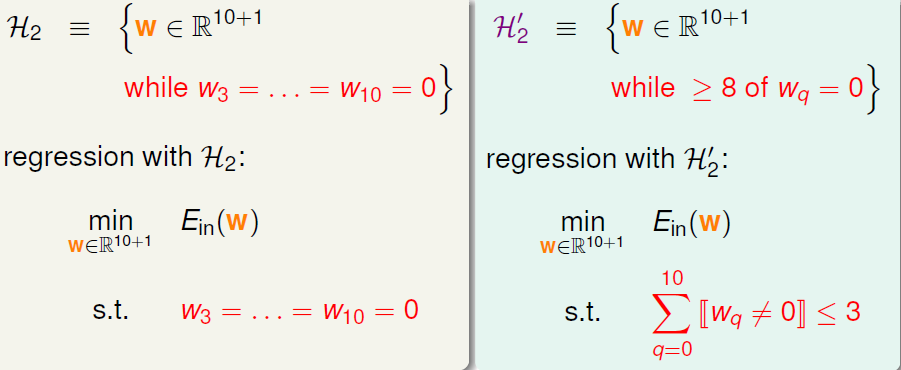
\includegraphics[width=12cm, height=4cm]{lecture14_1}\\
\end{center}
直接限制$W$个数,优化是$NP$,bad news for \textcolor{mypink3}{sparse hypothesis Set}.因此可以Softer下。
\begin{center}
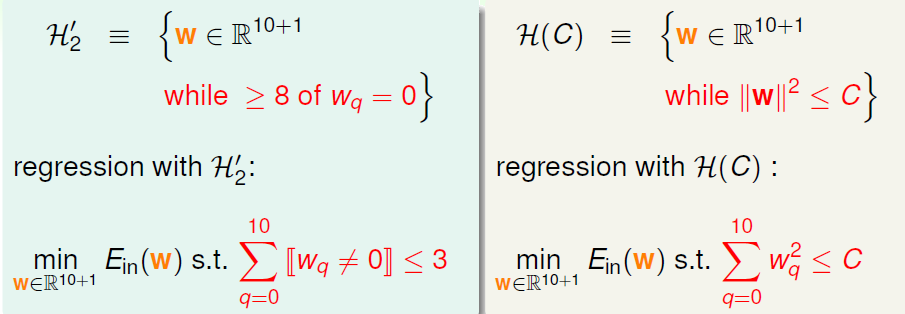
\includegraphics[width=12cm, height=4cm]{lecture14_2}\\
\end{center}

\subsection{Weight Decay Regularization} % (fold)
这样的意思就是把$W$现在在一个$\sqrt{C}$的圆里边。
\begin{align*}
\underset{w \in \mathbb{R}^{Q+1}}{\min} \ &E_{in}(w) = \frac{1}{N}\sum_{n=1}(w^Tz-y)^2 \\
s.t. \quad &\underbrace{\sum_{q=0}w_q^2}_{w^Tw} \leq C
\end{align*}
负的梯度方向可以垂直分解为圆的切线和法线方向。但是$C$限制了法线方向因此只能沿着圆的切线方向移动。因此$W_{reg}$的最优解是:负的梯度方向和法线方向是平行的。 \par
\begin{center}
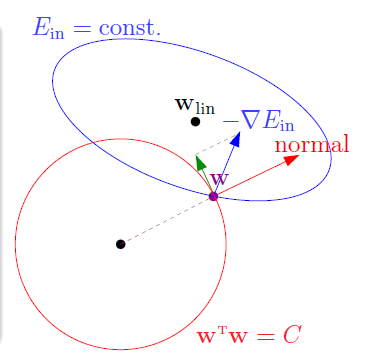
\includegraphics[width=5cm, height=5cm]{lecture14_3}\\
\end{center}
\begin{align*}
-\nabla{E_{in}{W_{reg}}} \propto W_{reg}
\end{align*}
使用有条件最优化工具Lagrange multiplier,可以模仿线性回归解正规方程了,也叫ridge regression。另外可以根据梯度公式推导出新的优化公式,这也是常见的L2正规化公式。\par
\begin{align*}
&\nabla{E_{in}(W) + \frac{2\lambda}{N}W} = 0 \\
&W \gets (Z^TZ + \lambda I)^{-1}Z^Ty \\
\end{align*}
\begin{align*}
solve \ \ &\nabla{E_{in}(W) + \frac{2\lambda}{N}W} = 0 \\
\underset{W}{\min} \quad &E_{in}(W) + \frac{\lambda}{N}\overbrace{W^TW}^{regular}
\end{align*}


\subsection{Regularization and VC Theory} % (fold)
\label{sub:regularization_and_vc_theory}

% subsection regularization_and_vc_theory (end)
\subsection{General Regularizers} % (fold)
\label{sub:general_regularizers}
\textbf{\textcolor{mypink2}{L2 and L1}}
\begin{center}
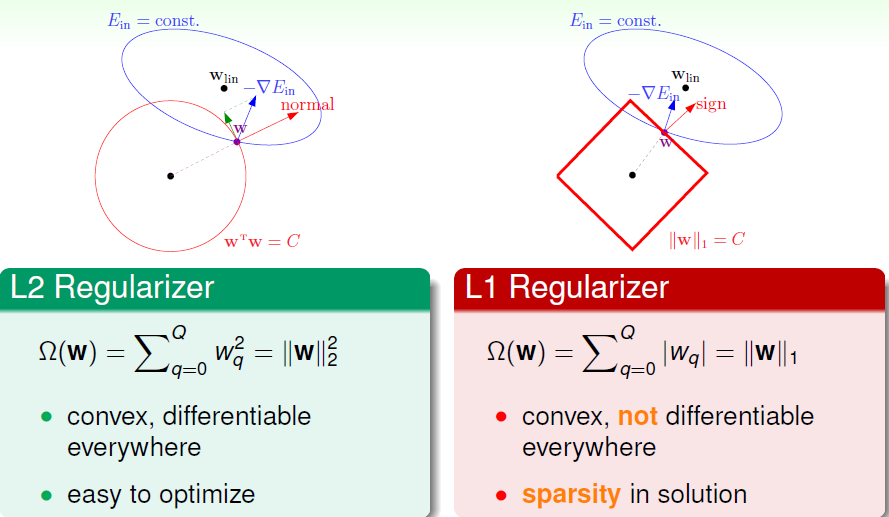
\includegraphics[width=10cm, height=7cm]{lecture14_4}\\
\end{center}
% subsection general_regularizers (end)
%%%%%%%%%%%%%%
\begin{center}
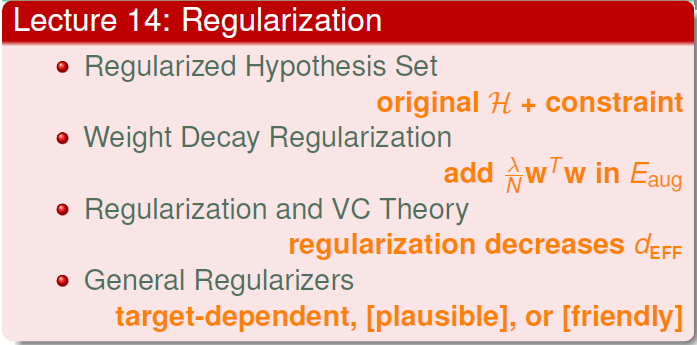
\includegraphics[width=10cm, height=5cm]{lecture14_sum}\\
\end{center}
\noindent
{\color{RubineRed} \rule{\linewidth}{1mm} }